\documentclass[a4paper,12pt,twoside]{article}
\usepackage[top=2.5cm,bottom=2.5cm,inner=3cm,outer=2cm, headheight=1.25cm, footskip=1.25cm]{geometry}
\usepackage{setspace}
\usepackage{fancyhdr}
\usepackage{titlesec}
\usepackage{enumitem}
\usepackage{hyperref}
\usepackage[polish]{babel}
\usepackage{pdfpages} % Dodaj pakiet pdfpages
\usepackage{graphicx}
\usepackage{float}
\usepackage[normalem]{ulem}
\usepackage[nottoc]{tocbibind}
\usepackage{courier}

%\hypersetup{colorlinks=true}

\usepackage[T1]{fontenc} % Użyj kodowania czcionek T1
\usepackage[utf8]{inputenc} % Użyj kodowania wejściowego UTF-8 dla znaków specjalnych
\usepackage{helvet} % Czcionka Helvetica
\usepackage{csquotes}
\renewcommand{\familydefault}{\sfdefault} % Ustaw domyślną czcionkę na bezszeryfową
\usepackage{amsmath} % Potrzebne do korzystania z środowisk matematycznych
\usepackage{chngcntr}
\counterwithin{figure}{section} % Numeracja rysunków zgodnie z numerem rozdziału
\counterwithin{table}{section}
\usepackage{amsmath}
\usepackage{tocloft}
\usepackage{nomencl}
\makenomenclature
\newcommand{\listequationsname}{\hspace{-1.0cm}\Large{Spis równań}}
\newlistof{myequations}{equ}{\listequationsname}
\newcommand{\myequations}[1]{%
    \addcontentsline{equ}{myequations}{\protect\numberline{\theequation}#1}\par
}

\usepackage{caption}
\captionsetup[figure]{name=Rys.}

\usepackage{listings}
\lstset{
    language=Python, % Wybierz język programowania
    basicstyle=\ttfamily, % Styl podstawowy
    numbers=left, % Numery linii po lewej stronie
    numberstyle=\tiny\color{gray}, % Styl numerów linii
    frame=single, % Rama wokół kodu
    breaklines=true, % Automatyczne łamanie linii
    captionpos=b, % Pozycja podpisu
    showstringspaces=false, % Nie pokazuj spacji w napisach
}

\usepackage{lmodern}
\renewcommand*\familydefault{\sfdefault}

\pagestyle{fancy}
\fancyhead{}
\fancyhead[LO,RE]{}
\fancyfoot{}
\fancyfoot[LE,RO]{\thepage}
\fancyfoot[LO,RE]{}
\renewcommand{\headrulewidth}{0pt}

\setlength{\parindent}{0.5cm}
\setlist[itemize]{label=•,itemsep=0pt}

\titleformat{\section}{\normalfont\fontsize{16}{18}\bfseries}{\thesection}{1em}{}
\titleformat{\subsection}{\normalfont\fontsize{14}{16}\bfseries}{\thesubsection}{1em}{}
\titleformat{\subsubsection}{\normalfont\fontsize{13}{15}\bfseries}{\thesubsubsection}{1em}{}

\newcommand{\MMp}[1]{\marginpar{\textcolor{blue}{\textbf{MM}: \footnotesize #1}}}
\newcommand{\MM}[1]{\textcolor{blue}{\textbf{MM}: #1}}

\usepackage[backend=bibtex,style=ext-authoryear,natbib=true]{biblatex}
\addbibresource{literatura.bib}

\DeclareOuterCiteDelims{cite}{\bibopenbracket}{\bibclosebracket}

\fancypagestyle{plain}{
    \fancyhf{} % Usuń wszystko z nagłówka i stopki
    \fancyfoot[LE,RO]{\thepage} % Dodaj numer strony na zewnętrznych krawędziach stopki
    \renewcommand{\headrulewidth}{0pt} % Brak linii w nagłówku
    \renewcommand{\footrulewidth}{0pt} % Brak linii w stopce
}

\fancypagestyle{empty}{
    \fancyhf{} % Usuń wszystko z nagłówka i stopki
    \renewcommand{\headrulewidth}{0pt} % Brak linii w nagłówku
    \renewcommand{\footrulewidth}{0pt} % Brak linii w stopce
}



\begin{document}

\newcommand{\codetext}[1]{{\fontfamily{pcr}\selectfont #1}}
\newcommand{\figMax}[3]{
        \begin{figure}[!h]
            \centering            \includegraphics[width=1\textwidth]{#1}
            \caption{#2}
            \label{#3}
        \end{figure}
	}
    
\newcommand{\figSAdjust}[3]{
        \begin{figure}[!h]
            \centering            \includegraphics[width=0.9\textwidth]{#1}
            \caption{#2}
            \label{#3}
        \end{figure}
	}
\newcommand{\figScale}[4]{
        \begin{figure}[H]
            \centering            \includegraphics[width=#4\textwidth]{#1}
            \caption{#2}
            \label{#3}
        \end{figure}
	}
\newcommand{\figScaleAdjust}[4]{
        \begin{figure}[!h]
            \centering            \includegraphics[width=#4\textwidth]{#1}
            \caption{#2}
            \label{#3}
        \end{figure}
	}
\newcommand{\figS}[3]{
        \begin{figure}[H]
            \centering            \includegraphics[width=0.9\textwidth]{#1}
            \caption{#2}
            \label{#3}
        \end{figure}
	}

\counterwithin{lstlisting}{section}
\thispagestyle{empty}


\includegraphics[width=5in]{LogoPL-FTIMS.pdf}

\begin{centering}

\vspace{1cm}

\textbf{\textit{\large{Aneta Malinowska}}}

\vspace{.1cm}

\textbf{\textit{\large{259279}}}

\vspace{1.5cm}

{\large{PRACA DYPLOMOWA}}

\vspace{.1cm}

{\large{magisterska}}

\vspace{.1cm}

na kierunku Informatyka Stosowana

\vspace{1.8cm}

\textbf{\Large{Automatyzacja personalizowanego planowania zadań z~uwzględnieniem zmęczenia i rytmu dobowego}}

\end{centering}

\vspace{2.25cm}
\begin{centering}
{Instytut Informatyki I72}\\
\end{centering}
\vspace{.25cm}
\textbf{Promotor:} dr inż. Joanna Ochelska-Mierzejewska

% \begin{centering}
% (tytuł/stopień naukowy, imię i nazwisko)

% ~\\

% \end{centering}
% \textbf{Opiekun pomocniczy:*)} \dotfill

% \begin{centering}
% (tytuł/stopień naukowy, imię i nazwisko)

% ~\\

% \end{centering}
% \textbf{Promotor uczelni partnerskiej:**)} \dotfill

% \begin{centering}
% (tytuł/stopień naukowy, imię i nazwisko)

% ~\\

% \end{centering}

\vfill

\begin{centering}
ŁÓDŹ 2026

\end{centering}
\hspace{0.5cm}
% \begin{itemize}
% \small
% \item[*]	jeśli został powołany
% \item[**]	w przypadku procedury uznania
% \end{itemize}
 % Wypełnij w tym pliku dane strony tytułowej
\pagenumbering{roman}
\setcounter{page}{2}
\newpage
\thispagestyle{empty}
\mbox{}
\newpage
\onehalfspacing

% Spis treści
% \pagestyle{empty}
\tableofcontents
\newpage
\clearpage

\pagestyle{fancy}
\pagenumbering{arabic}
\setcounter{page}{1}

% Rozdziały pracy
\newpage
\section*{Streszczenie}
% \addcontentsline{toc}{chapter}{Streszczenie}
\label{chap:Streszczenie}
%\addcontentsline{toc}{chapter}{Streszczenie}
%\markboth{STRESZCZENIE}{STRESZCZENIE}

% \quad Wraz z rosnącą liczbą kierunków studiów oferowanych przez uczelnie, kandydaci coraz częściej mają trudności z podjęciem dobrze poinformowanej decyzji dotyczącej wyboru kierunku. Aby rozwiązać ten problem, autorka opracowała program, który wykorzystuje techniki oceny osobowości i predyspozycji oraz metody uczenia maszynowego do zapewnienia spersonalizowanych rekomendacji kierunków studiów na Politechnice Łódzkiej. W tym celu wybrane zostały algorytmy filtrowania kolaboratywnego oraz \textit{LambdaRank}, powszechnie stosowane w systemach rekomendacji. Rozwiązanie zostało zaimplementowane jako aplikacja internetowa w formie quizu wielokrotnego wyboru, umożliwiając kandydatom otrzymanie dopasowanych rekomendacji na podstawie cech podobnych do aktualnych studentów. Aplikacja zbiera i przetwarza dane, aby wygenerować uporządkowaną listę proponowanych kierunków studiów, ułatwiając dostęp do istotnych informacji bez konieczności bezpośredniego kontaktu ze studentami. Ostatecznie przeanalizowano możliwe usprawnienia i strategie optymalizacji zaproponowanego rozwiązania, w tym ulepszenie zestawu pytań, rozszerzenie zbioru danych wykorzystywanego do trenowania modelu oraz zbadanie alternatywnych algorytmów rekomendacji. 

\bigskip
\section*{Abstract}
\label{chap:StreszczenieEng}
% \indent With the growing number of academic programs offered by universities, prospective students increasingly struggle to make well-informed decisions about their field of study. To address this issue, the author developed a program that utilizes personality and aptitude assessment techniques, along with machine learning methods, to provide personalized study program recommendations at Lodz University of Technology. Collaborative filtering algorithms and \textit{LambdaRank}, commonly used in recommendation systems, were selected for this purpose. The solution is~implemented as a web application in the form of a multiple-choice quiz, allowing candidates to~receive tailored recommendations based on characteristics similar to those of current students. The application collects and processes data to generate ranked study program suggestions, improving accessibility to relevant information without requiring direct interaction with students. Finally, potential improvements and optimization strategies for the proposed solution were analyzed, including refining the question set, expanding the dataset used for model training, and exploring alternative recommendation algorithms.
\bigskip

\textbf{Słowa kluczowe}: \quad automatyzacja  \quad planowanie zadań \quad uczenie przez wzmacnianie \quad algorytm genetyczny \quad produktywność \quad rytm dobowy \quad personalizacja

\noindent\textbf{Keywords}: \quad automation  \quad task planning \quad reinforcement learning \quad genetic algorithm \quad productivity \quad circadian rhythm \quad personalization


\newpage
% \section*{Wstęp}
% \addcontentsline{toc}{section}{Wstęp}
% \label{chap:Wstęp}
% \markboth{WSTĘP}{WSTĘP}
\section{Wstęp}\label{section_entry}
\subsection{Problematyka i zakres pracy}\label{section_problem}

% \quad We współczesnych środowiskach zawodowych oraz akademickich regularnie obserwuje się wzrost oczekiwań dotyczących liczby i złożoności realizowanych zadań. Pomimo rosnącej presji efektywnościowej, wiele osób nie dysponuje narzędziami ani umiejętnościami pozwalającymi na skuteczne zarządzanie własnym czasem. Prowadzi to do chronicznego przebodźcowania, spadku efektywności, a w skrajnych przypadkach – do wypalenia zawodowego. Jednym z czynników wpływających na nieefektywne planowanie jest nieuwzględnianie zmiennej natury funkcjonowania człowieka, w tym zmian wydajnosci związanych z rytmem dobowym i koniecznością odpoczynku. W efekcie powielane są niekorzystne nawyki, zamiast świadomego wykorzystania wiedzy o własnym rytmie dobowym do optymalizacji pracy.
\quad We współczesnych środowiskach zawodowych oraz akademickich regularnie obserwuje się wzrost oczekiwań dotyczących liczby i złożoności realizowanych zadań. Jednocześnie skuteczne planowanie aktywności człowieka stanowi złożony problem, ponieważ jego wydajność nie jest wartością stałą i może zmieniać się w zależności od czynników wewnętrznych i zewnętrznych. W szczególności znaczenie mają zmęczenie, potrzeba odpoczynku, rytm dobowy oraz indywidualne różnice w sposobie funkcjonowania. Nieuwzględnianie tej zmienności może prowadzić do tworzenia planów niedostosowanych do rzeczywistych możliwości użytkownika, a w konsekwencji do spadku efektywności, narastania obciążenia oraz powielania negatywnych nawyków.
% \\\indent Odpowiedzią na te wyzwania mogą być inteligentne systemy wspomagania decyzji, automatyzujące proces harmonogramowania w sposób spersonalizowany. Nowoczesne rozwiązania tego typu nie ograniczają się jedynie do sztywnych parametrów samych zadań (takich jak terminy czy priorytety). Opierają one swoje decyzje na modelowaniu zachowań użytkownika, analizie informacji zwrotnej o faktycznej użyteczności planu oraz iteracyjnej adaptacji algorytmów w czasie. Pozwala to na dostosowywanie systemu do indywidualnych cech użytkownika oraz obserwowanej zmienności jego wydajności w czasie.
\\\indent Odpowiedzią na te wyzwania mogą być inteligentne systemy wspomagania decyzji, automatyzujące proces harmonogramowania w sposób spersonalizowany. W przeciwieństwie do klasycznych metod opartych na sztywnych parametrach i wcześniej zdefiniowanych regułach, rozwiązania adaptacyjne mogą uwzględniać zmiany stanu użytkownika, jego historyczną wydajność oraz informacje zwrotne dotyczące realizacji planu. Pozwala to na bieżące dostosowywanie harmonogramu do indywidualnych cech użytkownika oraz zmienności jego funkcjonowania w czasie.
% \\\indent Choć metody automatycznego planowania są szeroko rozwijane w kontekście procesów systemowych czy interakcji człowiek-maszyna w przemyśle, istnieje wyraźna luka w ich adaptacji do dynamicznego i zróżnicowanego środowiska, jakim jest codzienne życie człowieka. 
\\\indent Choć metody automatycznego planowania są szeroko rozwijane w kontekście procesów systemowych, produkcyjnych czy współpracy człowieka z maszyną, ich zastosowanie w codziennym, indywidualnym planowaniu zadań nadal pozostaje ograniczone. Istotnym problemem jest również sposób reprezentowania czynników ludzkich, takich jak zmęczenie i regeneracja. W części istniejących rozwiązań odpoczynek traktowany jest jako aktywny element planu, jednak w wielu przypadkach jego wpływ na stan użytkownika nie jest jawnie modelowany.
% \\\indent Niniejsza praca podejmuje tę tematykę poprzez formalizację wpływu zmęczenia, rytmu dobowego oraz przerw na procesy decyzyjne. Zakres pracy obejmuje przegląd literatury i identyfikację metod optymalizacyjnych oraz podejść opartych na sztucznej inteligencji. W ramach badań opracowany i zaimplementowany zostanie jednolity model problemu planowania, który pozwoli na przeprowadzenie eksperymentów porównawczych wybranych algorytmów pod kątem efektywności oraz zgodności harmonogramu z przyjętymi ograniczeniami psychofizycznymi użytkownika.
\\\indent Niniejsza praca podejmuje tę tematykę poprzez formalizację wpływu rytmu dobowego, chronotypu, narastającego zmęczenia oraz regeneracji podczas odpoczynku na proces planowania zadań. Zakres pracy obejmuje analizę istniejących metod automatycznego harmonogramowania oraz opracowanie modelu symulacyjnego użytkownika, umożliwiającego prowadzenie eksperymentów porównawczych dla wybranych algorytmów w jednolitych warunkach.

% \newpage
\subsection{Cele pracy}\label{section_goals}

% \quad Głównym celem pracy jest opracowanie oraz eksperymentalna ocena wybranych metod automatycznego planowania zadań, z ukierunkowaniem na personalizację harmonogramu dla konkretnego użytkownika. W szczególności analizowany jest wpływ rytmu dobowego, zmienność funkcjonowania użytkownika w czasie pod wpływem narastającego zmęczenia i regeneracji w czasie odpoczynku. W związku z tym kluczowe jest zapoznanie się z metodami modelowania poziomów energii oraz wydajności człowieka z uwzględnieniem różnych chronotypów, a także dobór inteligentnych metod harmonogramowania umożliwiających operowanie na wielu zmiennych.
% \\\indent W celu zapewnienia jednolitych warunków porównania opracowany zostanie model symulacyjny użytkownika umożliwiający reprezentację różnych profili funkcjonowania oraz ich reakcji na wykonywanie zadań i odpoczynek. Na tej podstawie przeprowadzone zostanie porównanie modeli planistycznych dedykowanych dla jednostek z wykorzystaniem zdefiniowanych scenariuszy i miar jakośći. Eksperyment zostanie zrealizowany na bazie augmentowanych, ogólnodostępnych danych, co zapewni uproszczenie oraz weryfikowalność całego procesu.
% \\\indent Dodatkowym celem jest ocena wyników uzyskanych przez wybrane metody planowania pod kątem ich dostosowania do dynamicznego środowiska, potrzeb konkretnych użytkowników, narzuconych ograniczeń zadań oraz reakcji na zakłócenia, w oparciu o zdefiniowane miary efektywności.
\quad Głównym celem pracy jest opracowanie oraz eksperymentalna ocena wybranych metod automatycznego planowania zadań, z ukierunkowaniem na personalizację harmonogramu dla konkretnego użytkownika. W szczególności analizowany jest wpływ rytmu dobowego oraz zmienności funkcjonowania użytkownika w czasie, wynikającej z narastającego zmęczenia i regeneracji zachodzącej podczas odpoczynku. W związku z tym kluczowe jest zapoznanie się z metodami modelowania poziomu energii i wydajności człowieka z uwzględnieniem różnych chronotypów, a także dobór inteligentnych metod harmonogramowania umożliwiających uwzględnienie wielu zmiennych opisujących zarówno użytkownika, jak i realizowane zadania.
\\\indent W celu zapewnienia jednolitych warunków porównania opracowany zostanie model symulacyjny użytkownika, umożliwiający reprezentację różnych profili funkcjonowania oraz ich reakcji na wykonywanie zadań i odpoczynek. Na tej podstawie przeprowadzone zostanie porównanie wybranych modeli planistycznych dostosowanych do poszczególnych profili użytkowników, z wykorzystaniem zdefiniowanych scenariuszy badawczych oraz miar jakości. Eksperyment zostanie zrealizowany na bazie augmentowanych, ogólnodostępnych danych, co pozwoli na uproszczenie przygotowania środowiska badawczego oraz zapewnienie weryfikowalności całego procesu.
\\\indent Dodatkowym celem pracy jest ocena wyników uzyskanych przez wybrane metody planowania pod kątem ich zdolności do dostosowania się do dynamicznego środowiska, potrzeb konkretnych użytkowników, narzuconych ograniczeń związanych z zadaniami oraz pojawiających się zakłóceń. Ocena zostanie przeprowadzona w oparciu o zdefiniowane miary efektywności, pozwalające na porównanie jakości generowanych harmonogramów oraz stopnia ich dopasowania do przyjętego modelu funkcjonowania użytkownika.

\subsection{Układ pracy}\label{section_layout}
\quad Praca została podzielona na [X] rozdziałów.  W pierwszym przedstawiono problematykę badawczą oraz cele pracy, a także dokonano przeglądu literatury w zakresie automatyzacji planowania zadań oraz modelowania energii człowieka i rytmu dobowego. Drugi rozdział przedstawia teoretyczne wprowadzenie do rozważanego problemu oraz omówienie wybranych metod. W następnych rozdziałach omówiono kolejno strukturę danych oraz konstrukcję modeli i przeprowadzanego eksperymentu. Ostatecznie w rozdziałach \ref{section_results} i \ref{section_summary} przedstawiono i omówiono wyniki, przeprowadzając ocenę skuteczności wybranych metod, a także uwzględniono możliwe rozwinięcie tematyki personalizowanego planowania zadań. 
% Praca została podzielona na siedem rozdziałów. W pierwszym przedstawiono problematykę badawczą oraz cele pracy, a także dokonano przeglądu literatury dotyczącej systemów rekomendacyjnych. Drugi rozdział zawiera opis wybranych algorytmów oraz podstawowe zagadnienia związane z rekomendacjami. W kolejnym rozdziale przeanalizowano i porównano dostępne aplikacje służące do rekomendacji kierunków studiów. Rozdział czwarty opisuje technologie wykorzystane przy implementacji opracowanego systemu, natomiast piąty szczegółowo omawia proces jego tworzenia, poszczególne komponenty oraz funkcjonalności. Szósty rozdział pełni rolę podręcznika użytkownika, zawierając dokładny opis interfejsu aplikacji, a siódmy stanowi podsumowanie projektu, omawia uzyskane rezultaty oraz wskazuje możliwości dalszego rozwoju. 


\newpage
\section{Przegląd literatury}\label{section_literature}
\quad Niniejszy rozdział przedstawia przegląd literatury stanowiący podstawę do opracowania proponowanego rozwiązania oraz zdefiniowania modelu użytkownika wykorzystywanego w dalszej części pracy. Ze względu na interdyscyplinarny charakter badanego problemu analiza została podzielona na dwa uzupełniające się obszary. Pierwszy z nich obejmuje literaturę z zakresu automatyzacji i personalizacji planowania zadań, ze szczególnym uwzględnieniem metod optymalizacyjnych, uczenia przez wzmacnianie oraz podejść uwzględniających czynniki ludzkie. Część ta została opracowana w formie systematycznego przeglądu literatury, którego celem było uporządkowanie aktualnego stanu badań, identyfikacja dominujących metod oraz wskazanie ograniczeń istniejących rozwiązań.
\\\indent Druga część rozdziału koncentruje się na zagadnieniach związanych z funkcjonowaniem człowieka, w szczególności rytmem dobowym, chronotypem, zmęczeniem, regeneracją oraz zmiennością wydajności w czasie. Ze względu na pomocniczy charakter tego obszaru względem głównego problemu badawczego zastosowano ukierunkowany przegląd literatury, którego celem jest identyfikacja mechanizmów i zależności istotnych z punktu widzenia budowy modelu symulacyjnego użytkownika, w kontekście systemu harmonogramującego.
\\\indent Synteza obu obszarów pozwala następnie na sformułowanie założeń projektowanego rozwiązania i przejście do jego formalizacji oraz implementacji.

\subsection{Automatyzacja i personalizacja planowania zadań}

    \subsubsection{Metodyka systematycznego przeglądu literatury}
\quad Systematyczny przegląd literatury (ang. \textit{Systematic Literature Review}, SLR) to rygorystyczna metoda prowadzenia badań wtórnych, która wykorzystuje zdefiniowaną metodologię do identyfikacji, analizy i interpretacji dostępnych badań istotnych dla konkretnego obszaru badawczego lub zjawiska \cite{kitchenham2007guidelines}. W kontekście niniejszej pracy, proces ten pozwolił na obiektywne spojrzenie na problematykę personalizowanego harmonogramowania zadań. Cały proces badawczy składał się z trzech kluczowych faz:

\begin{enumerate}
    \item \textbf{Planowanie przeglądu}: celem tego etapu było sformułowanie pytań badawczych (RQ) oraz zdefiniowanie procedury selekcji. To tutaj określono zakres badań, skupiając się na kwestii optymalizacji algorytmicznej (GA, RL) oraz uwzględnienia w niej psychologii pracy (zmęczenie, prokrastynacja).
    
    \item \textbf{Realizacja przeglądu}: głównym zadaniem w tej fazie było opracowanie strategii wyszukiwania dla wybranych baz danych (ACM, IEEE, Science@Direct, Springer Link). Etap ten obejmował pozyskanie 157 pierwotnych studiów, a następnie ich wielostopniową ocenę. W wyniku rygorystycznej selekcji tytułów, abstraktów oraz oceny jakościowej (\textit{Quality Assessment}), wyłoniono finalny zbiór 22 publikacji, które stanowią podstawę do odpowiedzi na postawione pytania badawcze.
    
    \item \textbf{Raportowanie przeglądu}: ostatni etap polegał na syntezie zebranych danych i sformułowaniu wniosków w ujednoliconym formacie. Wynikiem tej fazy jest niniejszy rozdział, który systematyzuje wiedzę na temat trendów w \textit{AI-driven scheduling} i wskazuje kierunki dalszego rozwoju systemów wspierających produktywność osobistą.
\end{enumerate}

    \subsubsection{Pytania badawcze przeglądu}
    \quad Praca ta stara się przedstawić źródła i obserwowane w nich trendy w temacie personalizowanej automatyzacji zadań. W tym celu praca stara się odpowiedzieć na postawione pytania badawcze (RQ) zaprezentowane w tabeli \ref{tab:research_questions}. 


\begin{table}[h!]
\caption{Pytania badawcze (\textit{Research Questions}) sformułowane na potrzeby przeglądu.}\label{tab:research_questions}       
\begin{tabular}{p{0.8cm}p{14.4cm}}
\hline
\textbf{ID} & \textbf{Pytanie badawcze (\textit{Research Question})} \\ \hline
\textbf{RQ1} & Jakie są obecne podstawy algorytmiczne w personalizowanym planowaniu zadań i jak wybrane metody (GA, RL, agenci AI) wypadają w bezpośrednim porównaniu? \\ \hline
\textbf{RQ2} & Jakie parametry i ograniczenia skoncentrowane na użytkowniku (np. zmęczenie, przerwy, rytm okołodobowy) są najczęściej włączane do omawianych modeli? \\ \hline
\textbf{RQ3} & W jaki sposób dane o historycznej wydajności użytkownika (np. średni czas realizacji zadań) są wykorzystywane do personalizacji przyszłych przewidywań w harmonogramie? \\ \hline
\textbf{RQ4} & Jakie są główne metody weryfikacji, wyzwania oraz ograniczenia zidentyfikowane w~aktualnych rozwiązaniach dotyczących planowania zadań? \\ \hline
\end{tabular}
\end{table}

    \subsubsection{Strategia wyszukiwania}
    \quad Strategia wyszukiwania opierała się na serii zapytań przeprowadzonych w czterech cyfrowych bazach danych: ACM Digital Library, IEEE Digital Library, Science@Direct oraz Springer Link. W celu precyzyjnego sformułowania pytań badawczych i określenia zakresu przeglądu, wykorzystano metodę PICOC (\textit{Population, Intervention, Comparison, Outcome, Context}), która pozwoliła na zdefiniowanie następujących ram badania:

\begin{itemize}
    \item \textbf{Populacja (\textit{Population}):} Publikacje naukowe raportujące systemy planowania i harmonogramowania zadań, ze szczególnym uwzględnieniem modeli adaptowalnych dla indywidualnych użytkowników lub małych zespołów.
    \item \textbf{Interwencja (\textit{Intervention}):} Technologie i algorytmy optymalizacyjne, w szczególności algorytmy genetyczne (GA), uczenie przez wzmacnianie (RL) oraz agenci AI wykorzystywani do generowania harmonogramów zadań.
    \item \textbf{Porównanie (\textit{Comparison}):} Pozyskane badania nie są bezpośrednio porównywane z grupą kontrolną, jednak analiza skupia się na porównaniu wydajności różnych podejść AI (np. GA vs. RL) pod kątem ich zdolności adaptacyjnych.
    \item \textbf{Wyniki (\textit{Outcomes}):} Kluczowe parametry obejmują efektywność algorytmów, metryki produktywności, uwzględnienie ograniczeń dotyczących odpoczynku i przerw oraz zdolność systemu do dynamicznego dostosowania się do spersonalizowanego tempa pracy użytkownika.
    \item \textbf{Kontekst (\textit{Context}):} Systemy produktywności osobistej, inżynieria oprogramowania oraz szeroko pojęte środowiska IT, w których efektywne zarządzanie czasem i dobrostan pracownika są kluczowe.
\end{itemize}

\quad Mając powyższe na uwadze, po przeprowadzeniu iteracyjnych testów, zdefiniowano następujący ciąg wyszukiwania (ang. \textit{search string}) do odpytania wybranych baz danych:

\begin{quote}
\textit{(``task scheduling'' OR ``task planning'' OR ``time management'') AND (``genetic algorithm'' OR ``reinforcement learning'' OR ``AI agent'' OR ``intelligent agent'') AND (``personalization'' OR ``fatigue'' OR ``rest'' OR ``human factors'')}
\end{quote}

    
\subsubsection{Warunki uwzględnienia i wykluczenia}
\quad W celu filtrowania wyników wyszukiwania uzyskanych z baz danych postawiono warunki uwzględniania (IC) i wykluczenia (EC) prac, zaprezentowane kolejno w~tabeli~\ref{tab:inclusion_criteria} i tabeli~\ref{tab:exclusion_criteria}.


\begin{table}[h!]
\caption{Warunki uwzglednienia prac w przeglądzie}\label{tab:inclusion_criteria}       
\begin{tabular}{p{0.8cm}p{14.4cm}}
\hline
\textbf{ID} & \textbf{Warunek} \\ \hline
\textbf{IC1} & Pełne badania o przynajmniej 5 stronach. \\ \hline
\textbf{IC2} & Badania odpowiadające na przynajmniej jedno pytanie badawcze. \\ \hline
\textbf{IC3} & Prace podające praktyczne rozwiązania AI lub algorytmiczne. \\ \hline
\textbf{IC4} & Prace opublikowane w latach 2020-2026. \\ \hline
\end{tabular}
\end{table}

\begin{table}[h!]
\caption{Warunki wykluczenia prac z przeglądu}\label{tab:exclusion_criteria}       
\begin{tabular}{p{0.8cm}p{14.4cm}}
\hline
\textbf{ID} & \textbf{Warunek} \\ \hline
\textbf{EC1} & Duplikaty prac w różnych bazach. \\ \hline
\textbf{EC2} & Szara literatura. \\ \hline
\textbf{EC3} & Prace niepowiązane z tematem planowania zadań. \\ \hline
\textbf{EC4} & Prace z przed 2020 roku. \\ \hline
\textbf{EC5} & Prace w języku innym niż Polski lub Angielski. \\ \hline
\end{tabular}
\end{table}

\subsubsection{Ocena jakości (\textit{Quality Assessment})}\label{sec:QA}

\quad Po wstępnym filtrowaniu 26 wybranych prac poddano rygorystycznej ocenie jakościowej przy użyciu zestawu ośmiu pytań kontrolnych (QA), na które odpowiadano w skali: Tak (1 pkt), Częściowo (0.5 pkt), Nie (0 pkt). 

Pytania oceniające obejmowały:
\begin{enumerate}
    \item Czy badanie w sposób jawny modeluje ograniczenia ludzkie (zmęczenie, przerwy, rytm okołodobowy)?
    \item Czy oceniono zdolność algorytmu do adaptacji w dynamicznym środowisku?
    \item Czy algorytm harmonogramowania został jasno opisany?
    \item Czy praca wnosi wkład w personalizację produktywności?
    \item Czy cele i zakres badania są jasno określone?
    \item Czy omówiono ograniczenia proponowanego podejścia?
    \item Czy wyniki są poparte eksperymentami lub symulacjami?
    \item Czy kontekst badania (przemysł vs nauka) został odpowiednio opisany?
\end{enumerate}

Do ostatecznej syntezy danych dopuszczono wyłącznie prace, które uzyskały wynik powyżej 4.5 punktu. W rezultacie finalny zbiór badań podstawowych (ang. \textit{primary studies}) wyniósł 22 artykuły.



\subsubsection{Procedura selekcji}
\quad Przeszukanie baz danych za pomocą zdefiniowanego ciągu wyszukiwania zaowocowało zbiorem 157 publikacji. Rozkład prac pomiędzy poszczególne źródła prezentował się następująco: 85 (54.1\%) prac z bazy ACM Digital Library, 68 (43.3\%) z Science@Direct, 3 (1.9\%) z IEEE Digital Library oraz 1 (0.6\%) ze Springer Link (Rys. \ref{fig:articles_per_source}).

\begin{center}
\begin{figure}
\centering
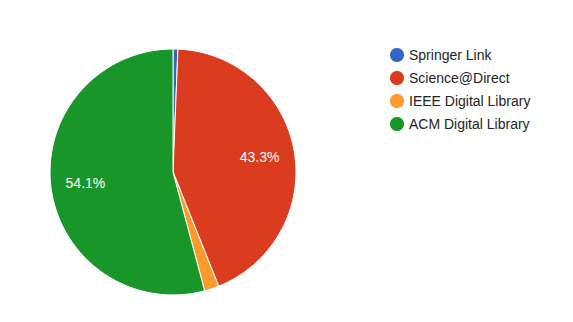
\includegraphics[scale=.65]{przeglad/art_per_src.png}
%
% If no graphics program available, insert a blank space i.e. use
%\picplace{5cm}{2cm} % Give the correct figure height and width in cm
%
\caption{Rozkłąd artykułów na poszczególne źródła}
\label{fig:articles_per_source}       % Give a unique label
\end{figure}
\end{center}

Zgromadzone prace zostały przefiltrowane w czterech etapach:
\begin{enumerate}
    \item \textbf{Wyszukiwanie wstępne:} zgromadzenie pełnej puli tekstów na podstawie słów kluczowych (157 prac).
    \item \textbf{Usuwanie duplikatów:} identyfikacja i usunięcie powtarzających się rekordów pomiędzy bazami (w analizowanym zbiorze nie zidentyfikowano duplikatów ze względu na specyficzne filtry baz).
    \item \textbf{Selekcja na podstawie tytułów i abstraktów:} zastosowanie kryteriów włączenia i wyłączenia do metadanych artykułów. Na tym etapie odrzucono prace dotyczące wyłącznie szeregowania procesów systemowych lub chmurowych, pozostawiając 26 publikacji.
    \item \textbf{Selekcja na podstawie pełnej treści i oceny jakości (QA):} szczegółowa lektura tekstów oraz ocena według 8 pytań kontrolnych (rozdział \ref{sec:QA}). Do końcowej analizy zakwalifikowano 22 prace, które przekroczyły próg punktowy 4,5.
\end{enumerate}


Po wstępnym filtrowaniu pozostało odpowiednio: 5 dla ACM, 19 dla Science@Direct, 1 dla IEEE oraz ok. 1 dla bazy Springer (Rysunek \ref{fig:articles_per_source_selected}).

\begin{figure}
\centering
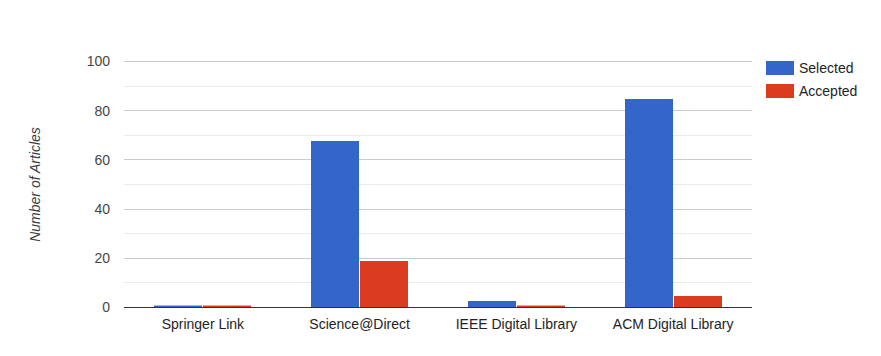
\includegraphics[scale=.4]{przeglad/art_per_src_selected.png}
\caption{Rozkład zaakceptowanych prac w porównaniu z początkowymi wynikami wyszukiwania}
\label{fig:articles_per_source_selected}       % Give a unique label
\end{figure}

Opisany proces, zilustrowany w tabeli \ref{tab:selection_stages}, pozwolił na wyłonienie najbardziej relewantnych badań pierwotnych odpowiadających na postawione pytania badawcze.

\begin{table}[h!]
\centering
\caption{Etapy selekcji artykułów i liczba prac zakwalifikowanych.}
\label{tab:selection_stages}
\begin{tabular}{p{5cm} c c c c c}
\hline
\textbf{Etap selekcji} & \textbf{ACM} & \textbf{Science@Direct} & \textbf{IEEE} & \textbf{Springer} & \textbf{Wszystkie} \\ \hline
Wyszukiwanie wstępne & 85 & 68 & 3 & 1 & 157 \\ \hline
Usuwanie duplikatów & 85 & 68 & 3 & 1 & 157 \\ \hline
Analiza tytułów i abstraktów & 5 & 19 & 1 & 1 & 26 \\ \hline
Pełna analiza treści (Finalny zbiór) & 2 & 18 & 1 & 1 & 22 \\ \hline
\end{tabular}
\end{table}

\subsubsection{Ekstrakcja i synteza danych}
\quad Ostatnim etapem fazy realizacji przeglądu było systematyczne pozyskanie danych z 22 zakwalifikowanych studiów pierwotnych. W tym celu opracowano formularz ekstrakcji danych (ang. \textit{Data Extraction Form}), którego strukturę zaprojektowano tak, aby bezpośrednio wspierała odpowiedzi na postawione pytania badawcze (RQ1-RQ4).

Formularz składał się z zestawu pól kategoryzujących aspekty techniczne algorytmów oraz specyficzne parametry uwzględniające czynnik ludzki. Szczegółowy opis pól formularza przedstawia Tabela~\ref{tab:data_extraction_form}.

\begin{table}[h!]
\caption{Struktura formularza ekstrakcji danych.}
\label{tab:data_extraction_form}
\begin{tabular}{p{4cm}p{2.2cm}p{8.4cm}}
\hline
\textbf{Pole danych} & \textbf{Typ danych} & \textbf{Uzasadnienie / Powiązanie z RQ} \\ \hline
Typ algorytmu & Kategoria & Klasyfikacja metod (GA, RL, Agenci AI, Inne). (\textbf{RQ1}). \\ \hline
Focus na personalizację & Boolean (T/N) & Ocena, czy model realnie adaptuje się do historii użytkownika. (\textbf{RQ3}). \\ \hline
Modelowanie odpoczynku & Kategoria & Rozróżnienie między aktywnym planowaniem przerw a pasywnym stanem bezczynności. (\textbf{RQ2}). \\ \hline
Metoda weryfikacji & Kategoria & Identyfikacja sposobu walidacji (Symulacja, Eksperyment z użytkownikami, Case Study). (\textbf{RQ4}). \\ \hline
Skalowalność & Boolean (T/N) & Ocena, czy rozwiązanie może być stosowane przy dużej liczbie zadań/użytkowników. (\textbf{RQ4}). \\ \hline
Główne wyzwanie & Tekstowe & Opis barier technologicznych lub psychologicznych (np. błąd planowania). (\textbf{RQ4}). \\ \hline
\end{tabular}
\end{table}


\indent Proces ekstrakcji został przeprowadzony przy użyciu narzędzia Parsifal, co zapewniło spójność danych. W przypadku pól kategorycznych (np. modelowanie odpoczynku), każda praca była analizowana pod kątem tego, czy przerwy w pracy są traktowane jako zaplanowany element regeneracji (\textit{active rest period}), czy jedynie jako brak zadań w systemie (\textit{passive idle}). Dane te posłużyły w dalszej części pracy do przeprowadzenia syntezy ilościowej i jakościowej.


    \subsubsection{Wyniki systematycznego przeglądu literatury}
    
\quad W tym rozdziale przedstawiono wyniki projektu badawczego przeprowadzonego na wybranych 22 pracach, które przedstawiono w tabeli \ref{tab:final_studies}. Każda z nich została poddana szczegółowej ekstrakcji danych pod kątem postawionych pytań badawczych.

\begin{table}[htbp!]
\caption{Zestawienie wybranych artykułów pierwotnych.}
\label{tab:final_studies}
\begin{tabular}{p{0.3cm}p{11.5cm}p{3cm}}
\hline
\textbf{ID} & \textbf{Tytuł artykułu} & \textbf{Wpis} \\ \hline
1 & Platform-based task assignment for social manufacturing (PBTA4SM): State-of-the-art review and future directions & \cite{PBTA4SM} \\ \hline
% 2 & Alert Fatigue in Security Operations Centres: Research Challenges and Opportunities & \cite{alert2025} \\ \hline
2 & From Conversation to Orchestration: HCI Challenges and Opportunities in Interactive Multi-Agentic Systems & \cite{orchestration2026} \\ \hline
3 & Dual task scheduling strategy for personalized multi-objective optimization of cycle time and fatigue in human-robot collaboration & \cite{dualTask2023} \\ \hline
4 & Task Allocation in Human-Robot Collaboration (HRC) Based on Task Characteristics and Agent Capability for Mold Assembly & \cite{HRC2020} \\ \hline
5 & An approach to task scheduling in an end-of-line quality assurance situation with human-robot cooperation & \cite{endline2025} \\ \hline
6 & Hierarchical online automated planning for a flexible manufacturing system & \cite{hierarchy2024} \\ \hline
7 & Towards a science exocortex & \cite{exocortex2024} \\ \hline
8 & JSHM: A dynamic flexible job-shop scheduling method with human-machine collaboration & \cite{JSHM2026} \\ \hline
9 & Tourist trip planning with priority discipline & \cite{tourist2025} \\ \hline
10 & Future-Proof Production Scheduling and Control & \cite{future2025} \\ \hline
11 & Real-time physical fatigue risk assessment for construction workers using a teacher-student training paradigm & \cite{fatigue2025} \\ \hline
12 & Education 4.0: Artificial Intelligence Assisted Task- and Time Planning System & \cite{education2022} \\ \hline
13 & A novel real-world human-robot collaboration scheduling problem: a combination of assembly line balancing and flow shop scheduling & \cite{novelHCR2025} \\ \hline
14 & Intelligent Time Management Recommendations Using Bayesian Optimization & \cite{bayesian2024} \\ \hline
15 & A reinforcement learning based algorithm for personalization of digital, just-in-time, adaptive interventions & \cite{inTimeRL2021} \\ \hline
16 & Can large language models independently complete tasks? A dynamic evaluation framework for multi-turn task planning and completion & \cite{LLM2025} \\ \hline
17 & Development of a new personalized staff-scheduling method with a work-life balance perspective: case of a hospital & \cite{workLifeBalance2023} \\ \hline
18 & Embracing open innovation in hospitality management: Leveraging AI-driven dynamic scheduling systems for complex resource optimization and enhanced guest satisfaction & \cite{hospitality2025} \\ \hline
% 20 & Self-organizing manufacturing network: A paradigm towards smart manufacturing in mass personalization & \cite{selfOrganizing2021} \\ \hline
% 21 & Artificial Intelligence Helps Teachers Personalise Their Teaching--Take ChatGPT as an Example & \cite{teachers2025} \\ \hline
19 & Bridging the Gap Between Time Management Research and Task Management App Design: A Study on the Integration of Planning Fallacy Mitigation Strategies & \cite{gap2024} \\ \hline
20 & Task Allocation in Human-Robot Collaboration: A Simulation-based approach to optimize Operator's Productivity and Ergonomics & \cite{TaskAllocation2024} \\ \hline
21 & Digital twin-based framework for an efficient execution of CPPS reconfiguration through human–robot collaboration & \cite{twin2025} \\ \hline
22 & A competence-time-quality scheduling model of multi-skilled staff for IT project portfolio & \cite{competenceTimeQuality2020} \\ \hline
% 26 & Voicing Suggestions and Enabling Reflection: Results of an Expert Discussion on Proactive Assistants for Time Management & \cite{Voicing2023} \\ \hline
\end{tabular}
\end{table}

\subsubsection{Opis badań podstawowych}
\quad Na potrzeby tego badania analizowane były jedynie prace z lat 2020-2026 w celu sprawdzenia aktualnych trendów i nowych rozwiązań dla problemów dynamicznego środowiska i uwzględnienia cech ludzkich w planowaniu. Liczność wybranych prac na przestrzeni lat została zaprezentowana na rysunku \ref{fig:articles_per_year} 

\begin{figure}[h!]
\centering
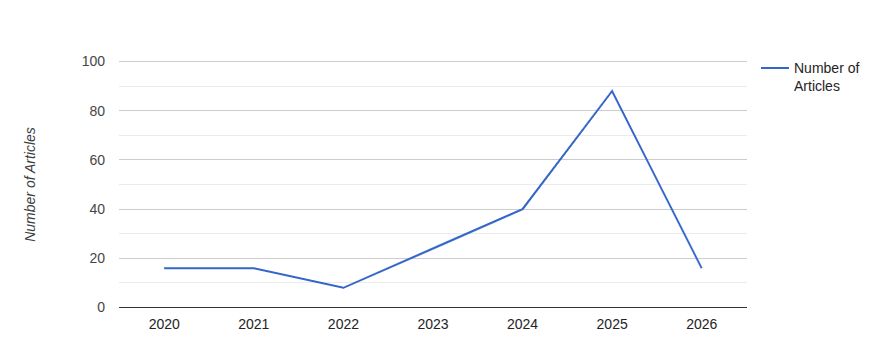
\includegraphics[scale=.38]{przeglad/art_per_year.png}
\caption{Rozkład liczności wybranych prac na przestrzeni lat.}
\label{fig:articles_per_year}      
\end{figure}

\subsubsection{Wykaz analizy jakości (\textit{Quality Assessment})}
\quad Na podstawie warunków przedstawionych w rozdziale \ref{sec:QA} oceniono wybrane prace w celu ustalenia ich wartości merytorycznej w kontekście tego badania, co zaprezentowano w tabeli \ref{tab:QA_res}. Średnia jakość prac to około 80\%. Na szczególną uwagę zasługują prace Hämmerle i in. \cite{endline2025} oraz Gönül i in. \cite{inTimeRL2021}, które jako jedyne uzyskały maksymalną ocenę w procesie \textit{Quality Assessment}. Prace te stanowią wzorzec metodologiczny, łącząc zaawansowane modele uczenia przez wzmacnianie (RL) z rygorystyczną weryfikacją w warunkach zbliżonych do rzeczywistych, przy jednoczesnym pełnym uwzględnieniu dynamiki ludzkiego zmęczenia.


\begin{table}[htbp!]
\caption{Zestawienie wybranych artykułów pierwotnych.}
\label{tab:QA_res}
\begin{tabular}{p{3cm} p{1cm} p{1cm} p{1cm} p{1cm} p{1cm} p{1cm} p{1cm} p{1cm} p{1cm}}
\hline
\textbf{ID} & \textbf{QA1} & \textbf{QA2} & \textbf{QA3} & \textbf{QA4} & \textbf{QA5} & \textbf{QA6} & \textbf{QA7} & \textbf{QA8} & \textbf{Razem} \\ \hline
1 \cite{PBTA4SM} & 0 & 0.5 & 0.5 & 0.5 & 1 & 1 & 0.5 & 1 & 5 \\ \hline
2 \cite{orchestration2026} & 0.5 & 1 & 0.5 & 0 & 1 & 1 & 0.5 & 1 & 5.5 \\ \hline
3 \cite{dualTask2023} & 1 & 0.5 & 1 & 1 & 1 & 0.5 & 1 & 1 & 7 \\ \hline
4 \cite{HRC2020} & 1 & 1 & 1 & 1 & 1 & 0.5 & 1 & 1 & 7.5 \\ \hline
5 \cite{endline2025} & 1 & 1 & 1 & 1 & 1 & 1 & 1 & 1 & 8 \\ \hline
6 \cite{hierarchy2024} & 0 & 1 & 1 & 0 & 1 & 0.5 & 1 & 1 & 5.5 \\ \hline
7 \cite{exocortex2024} & 1 & 1 & 0.5 & 1 & 1 & 1 & 0.5 & 1 & 7 \\ \hline
8 \cite{JSHM2026} & 1 & 1 & 1 & 1 & 1 & 0.5 & 1 & 1 & 7.5 \\ \hline
9 \cite{tourist2025} & 0.5 & 0.5 & 1 & 1 & 1 & 1 & 1 & 1 & 7 \\ \hline
10 \cite{future2025} & 0 & 1 & 1 & 0 & 1 & 0.5 & 1 & 1 & 5.5 \\ \hline
11 \cite{fatigue2025} & 1 & 1 & 1 & 1 & 1 & 0.5 & 1 & 1 & 7.5 \\ \hline
12 \cite{education2022} & 1 & 0.5 & 1 & 1 & 1 & 0.5 & 1 & 1 & 7 \\ \hline
13 \cite{novelHCR2025} & 0 & 0.5 & 1 & 0 & 1 & 0.5 & 1 & 1 & 5 \\ \hline
14 \cite{bayesian2024} & 0.5 & 1 & 1 & 1 & 1 & 0.5 & 1 & 1 & 7 \\ \hline
15 \cite{inTimeRL2021} & 1 & 1 & 1 & 1 & 1 & 1 & 1 & 1 & 8 \\ \hline
16 \cite{LLM2025} & 0 & 1 & 1 & 1 & 1 & 1 & 1 & 0.5 & 6.5 \\ \hline
17 \cite{workLifeBalance2023} & 1 & 0.5 & 1 & 1 & 1 & 0.5 & 1 & 1 & 7 \\ \hline
18 \cite{hospitality2025} & 0.5 & 1 & 0.5 & 0.5 & 1 & 0.5 & 0.5 & 1 & 5.5 \\ \hline
19 \cite{gap2024} & 1 & 0 & 0 & 1 & 1 & 0.5 & 0.5 & 1 & 5 \\ \hline
20 \cite{TaskAllocation2024} & 1 & 0.5 & 1 & 1 & 1 & 0.5 & 1 & 1 & 7 \\ \hline
21 \cite{twin2025} & 0.5 & 1 & 1 & 0.5 & 1 & 0.5 & 1 & 1 & 6.5 \\ \hline
22 \cite{competenceTimeQuality2020} & 0.5 & 0.5 & 1 & 0.5 & 1 & 0.5 & 1 & 1 & 6 \\ \hline
\end{tabular}
\end{table}


\subsubsection{RQ1: Jakie są obecne podstawy algorytmiczne w personalizowanym planowaniu zadań i jak wybrane metody (GA, RL, agenci AI) wypadaj ˛a w bezpośrednim porównaniu?}
\quad Analiza wykorzystanych technologii (rysunek \ref{fig:algo_dist}) wykazuje znaczną różnorodność w podejściu do problemu harmonogramowania, co świadczy o odejściu od prostych modeli statycznych na rzecz systemów wysoce adaptacyjnych. Choć literatura tradycyjna opiera się głównie na klasycznych algorytmach metaheurystycznych, w badaniach z lat 2020–2026 zauważalny jest wyraźny wzrost zainteresowania metodami dynamicznymi, zdolnymi do reagowania na zmienność ludzkiego działania w czasie rzeczywistym.

\begin{figure}[h!] 
	\centering 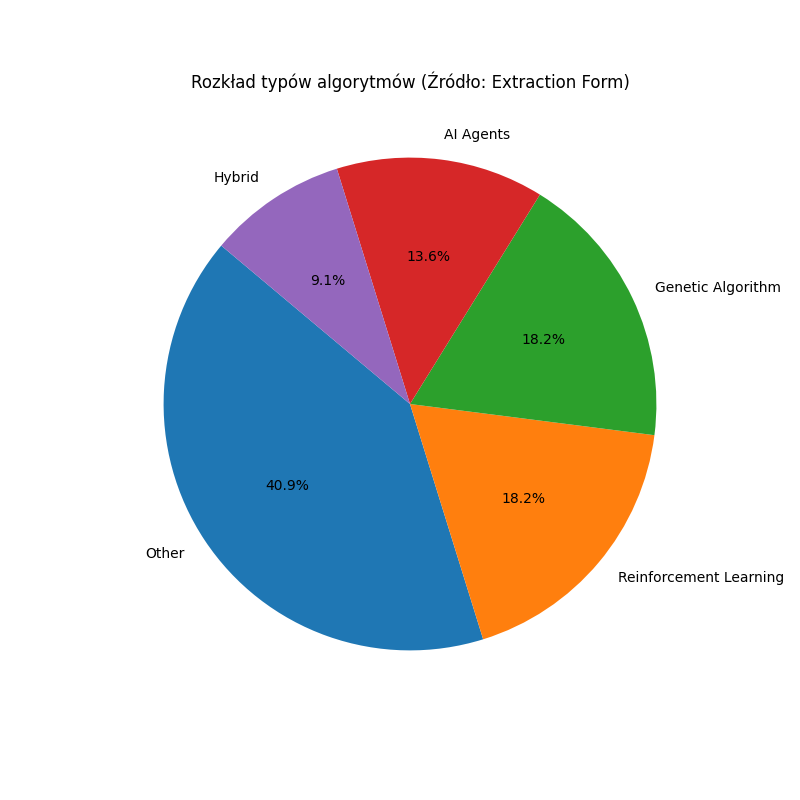
\includegraphics[width=0.7\textwidth]{przeglad/wykres_algorytmy.png} \caption{Rozkład typów algorytmów w analizowanych badaniach.} \label{fig:algo_dist} \end{figure}

\indent Jednym z kluczowych filarów technologicznych, zidentyfikowanym w 18,2\% analizowanych prac, jest uczenie przez wzmacnianie (\textit{Reinforcement Learning} - RL). Metoda ta znajduje zastosowanie przede wszystkim w scenariuszach, w których system musi uczyć się preferencji użytkownika na bieżąco i wdrażać interwencje typu \textit{Just-in-Time} \cite{inTimeRL2021}. Zaawansowane implementacje, takie jak model JSHM, łączą głębokie RL z wielozadaniowymi grafowymi sieciami neuronowymi (MBGCN), co pozwala na precyzyjne i jednoczesne modelowanie umiejętności operatora, stopnia trudności zadań oraz indywidualnych tendencji behawioralnych \cite{JSHM2026}.

\indent Równorzędne znaczenie pod względem częstotliwości występowania (18,2\% przypadków) zachowują algorytmy genetyczne (GA). W najnowszych badaniach rzadko występują one w swojej podstawowej formie; najczęściej są modyfikowane w celu zwiększenia ich wydajności w środowiskach dynamicznych. Ich rola koncentruje się głównie na optymalizacji wielokryterialnej, mającej na celu znalezienie stabilnego balansu między wydajnością systemu a poziomem zmęczenia człowieka \cite{dualTask2023}. Często spotyka się tu również hybrydy, łączące GA z algorytmami przeszukiwania lokalnego (np. \textit{Tabu Search}), co pozwala na skuteczne rozwiązywanie problemów synchronizacji w złożonych procesach współpracy \cite{novelHCR2025}.

\indent Kolejną istotną grupę, stanowiącą 13,6\% zbioru, tworzą Agenci AI. Badania w tym obszarze koncentrują się na proaktywnej komunikacji i orkiestracji działań w interaktywnych środowiskach wieloagentowych \cite{orchestration2026}. Agenci ci pełnią rolę kognitywnego rozszerzenia użytkownika – przykładem jest koncepcja „egzokortyksu naukowego”, w której rój agentów wspiera badacza w podejmowaniu decyzji i planowaniu długich łańcuchów zadań \cite{exocortex2024}.

\indent Najliczniejsza kategoria, obejmująca aż 41\% badanych rozwiązań (grupa „Inne i Hybrydy”), odzwierciedla dużą innowacyjność obecnych badań. W tej grupie dominują nowatorskie zastosowania dużych modeli językowych (LLM), które są oceniane pod kątem ich zdolności do samodzielnego planowania i wykonywania zadań w scenariuszach wieloetapowych \cite{LLM2025}. Ponadto analiza wskazuje na istotny wkład optymalizacji bayesowskiej w generowanie rekomendacji czasowych przy ograniczonych danych \cite{bayesian2024} oraz wykorzystanie architektur cyfrowych bliźniaków (\textit{Digital Twins}) opartych na sieciach neuronowych informowanych fizycznie (PINNs) do precyzyjnego przewidywania stanów systemu \cite{twin2025}. Tak szerokie spektrum metod potwierdza, że skuteczne, personalizowane planowanie wymaga łączenia zaawansowanej analityki danych z elastycznymi modelami decyzyjnymi.

\subsubsection{RQ2: Jakie parametry i ograniczenia skoncentrowane na użytkowniku (np. zmęczenie, przerwy, rytm okołodobowy) są najczęściej włączane do omawianych modeli?}
\quad Modelowanie ograniczeń ludzkich w analizowanej literaturze wykracza znacząco poza proste ramy czasowe, kładąc nacisk na procesy biologiczne, ergonomiczne i psychofizyczne. Kluczowym parametrem uwzględnianym w badaniach jest zmęczenie fizyczne oraz kognitywne, przy czym wyniki przeglądu wskazują na istotną i trwającą zmianę paradygmatu w podejściu do regeneracji sił użytkownika. 

\indent Obecnie \textbf{32\%} analizowanych prac implementuje koncepcję aktywnych przerw (\textit{active rest period}), w której odpoczynek nie jest traktowany jako zwykły przestój, lecz jako jawne zadanie regeneracyjne mające na celu czynne obniżenie poziomu zmęczenia (\textit{fatigue mitigation}). Podejście to jest szczególnie widoczne w pracach dotyczących współpracy człowiek-robot, gdzie optymalizacja czasu cyklu jest bezpośrednio powiązana z modelem wypoczynku operatora \cite{dualTask2023, endline2025}, a także w systemach monitorujących ryzyko fizyczne w czasie rzeczywistym \cite{fatigue2025, TaskAllocation2024}. Ponadto, aktywne planowanie interwencji w odpowiednich momentach spoczynku jest kluczowe dla skuteczności personalizowanych systemów zdrowotnych \cite{inTimeRL2021}.

\indent Mimo tego nowoczesnego trendu, \textbf{27\%} publikacji wciąż stosuje podejście pasywne (\textit{passive idle}), gdzie odpoczynek jest jedynie efektem braku dostępnych zadań w systemie, co często wynika ze specyfiki alokacji zadań opartej głównie na charakterystyce maszyn, a nie człowieka \cite{HRC2020, hierarchy2024}. 

\indent Warto zauważyć, że w \textbf{41\%} przypadków model odpoczynku nie został jawnie zdefiniowany, co wskazuje na potrzebę dalszych badań nad standaryzacją okresów regeneracji. Poza samym zmęczeniem, zaawansowane modele integrują parametry takie jak zasady \textit{work-life balance} \cite{workLifeBalance2023}, ergonomia postawy \cite{TaskAllocation2024} oraz indywidualna wydajność kognitywna, co pozwala na ochronę zdrowia przy zachowaniu efektywności.

\subsubsection{RQ3: W jaki sposób dane o historycznej wydajności użytkownika (np. średni czas realizacji zadań) są wykorzystywane do personalizacji przyszłych przewidywań w harmonogramie?}
\quad Dane historyczne stanowią fundament adaptacyjności systemów personalizowanych, umożliwiając ciągłe dostrajanie parametrów algorytmicznych do specyfiki konkretnego użytkownika. Jak wykazano w procesie ekstrakcji danych, aż \textbf{68\%} analizowanych prac (15 artykułów) wykazuje wyraźną koncentrację na zagadnieniu personalizacji (\textit{Personalization Focus}), co potwierdza trend odchodzenia od sztywnych systemów planistycznych na rzecz rozwiązań adaptacyjnych \cite{JSHM2026, bayesian2024}.

\indent Historia wydajności jest wykorzystywana przede wszystkim do modelowania indywidualnych krzywych uczenia się i zapominania, co pozwala systemowi przewidzieć tempo nabywania wprawy i skracać szacowany czas trwania kolejnych zadań \cite{competenceTimeQuality2020}. Dodatkowo, analiza historycznych różnic między założonym planem a rzeczywistym wykonaniem służy do łagodzenia skutków błędu planowania (\textit{planning fallacy}) poprzez automatyczną korektę przyszłych estymacji czasu \cite{gap2024}. Dzięki wysokiemu poziomowi personalizacji, algorytmy uczą się rzeczywistego tempa pracy użytkownika, co pozwala na unikanie przeciążenia informacyjnego i kognitywnego \cite{orchestration2026, inTimeRL2021}. Systemy te potrafią również przewidywać momenty skłonności do prokrastynacji, sugerując podział przytłaczających obowiązków na mniejsze etapy w oparciu o wcześniejsze sukcesy użytkownika w realizacji planu \cite{education2022}.


\subsubsection{RQ4: Jakie są główne metody weryfikacji, wyzwania oraz ograniczenia zidentyfikowane w aktualnych rozwiązaniach dotyczących planowania zadań?}

\quad Weryfikacja proponowanych rozwiązań w obszarze personalizowanego harmonogramowania opiera się na różnorodnych metodach badawczych, co zilustrowano na rysunku \ref{fig:verification_dist}. Wyniki przeglądu wskazują na wyraźną dominację symulacji, które zostały wykorzystane w 50\% analizowanych prac. Trend ten wynika przede wszystkim z łatwości generowania dużych i zróżnicowanych zbiorów danych testowych, co jest niezbędne do oceny wydajności złożonych algorytmów. Niepokojącym zjawiskiem pozostaje jednak relatywnie mała liczba eksperymentów z udziałem realnych użytkowników (\textit{User Experiments}), które stanowią jedynie 13,6\% zbioru. Taka dysproporcja sugeruje, że wiele współczesnych modeli zachowuje charakter teoretyczny i może napotykać trudności w bezpośrednim starciu z nieprzewidywalnymi zachowaniami ludzkimi w rzeczywistym środowisku pracy.

\begin{figure}[h!] \centering 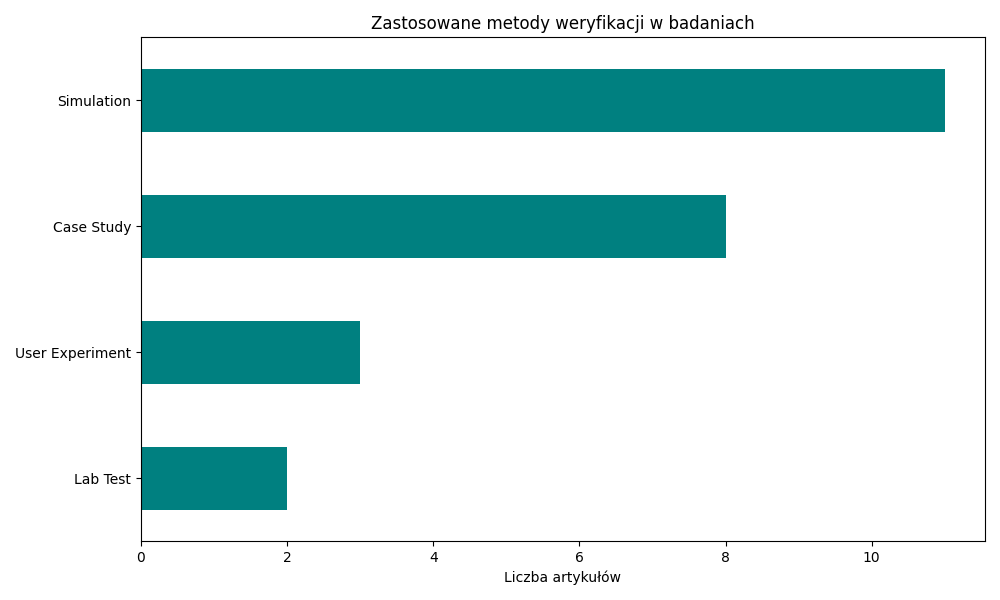
\includegraphics[width=0.8\textwidth]{przeglad/wykres_weryfikacja.png} \caption{Metody weryfikacji stosowane w analizowanych badaniach.} \label{fig:verification_dist} \end{figure}

\indent Pewną próbę wypełnienia luki między teorią a praktyką stanowią podejścia wykorzystujące technologie rzeczywistości mieszanej (MR) oraz cyfrowe bliźniaki. Przykładowo, integracja modułów MR z architekturą bliźniaka cyfrowego pozwala na bezpieczne testowanie interakcji człowiek-robot przy jednoczesnym zachowaniu wysokiej wierności odwzorowania warunków fizycznych \cite{twin2025}. W nielicznych eksperymentach z użytkownikami badacze koncentrują się nie tylko na twardych metrykach wydajności, ale również na subiektywnej satysfakcji, poziomie stresu oraz wskaźniku skutecznego ukończenia zadań \cite{education2022, bayesian2024}.

\indent Analiza literatury pozwoliła na zidentyfikowanie szeregu barier technologicznych i psychologicznych, które ograniczają skuteczność obecnych systemów. Jednym z najpoważniejszych wyzwań jest problem wyjaśnialności (\textit{explainability}) decyzji podejmowanych przez sztuczną inteligencję. Jak wskazują autorzy koncepcji asystentów kognitywnych, brak przejrzystego uzasadnienia, dlaczego system sugeruje zmianę planu lub konieczność odpoczynku, znacząco obniża zaufanie użytkownika i rygor przestrzegania wygenerowanego harmonogramu \cite{exocortex2024}. Wyzwaniem technicznym pozostaje również wykładniczy wzrost złożoności obliczeniowej w przypadku dużej liczby zadań \cite{hierarchy2024} oraz tendencja nowoczesnych modeli językowych (LLM) do gubienia kontekstu podczas planowania długofalowych procesów \cite{LLM2025}.

\indent Najważniejszym ograniczeniem o charakterze ludzkim pozostaje jednak błąd planowania (\textit{planning fallacy}) oraz związana z nim niska rzetelność danych wejściowych. Użytkownicy wykazują systematyczną tendencję do niedoszacowania czasu potrzebnego na realizację zadań, co prowadzi do dezaktualizacji harmonogramu już w początkowej fazie jego wykonywania \cite{gap2024}. Problem ten potęguje trudność w precyzyjnym i obiektywnym określaniu momentów zmęczenia ze względu na duże różnice międzyosobnicze \cite{fatigue2025}. W efekcie, kluczowym wyzwaniem dla przyszłych systemów pozostaje zapewnienie wysokiej odporności (\textit{robustness}) na zakłócenia oraz zdolność do ciągłej, dynamicznej rekonfiguracji planu bez powodowania nadmiernego obciążenia informacyjnego u użytkownika \cite{future2025, orchestration2026}.

\begin{table}[htbp!]
\caption{Szczegółowe zestawienie wyzwań badawczych dla każdej pracy; część 1}
\label{tab:challenges_summary}
\begin{tabular}{p{0.5cm} p{8cm}|p{6.3cm}}
\hline
\textbf{ID} & \textbf{Artykuł} & \textbf{Główne wyzwanie} \\ \hline
1 & Platform-based task assignment for social manufacturing (PBTA4SM): State-of-the-art review and future directions & Zapewnienie zaufania i bezpieczeństwa zdecentralizowanej sieci. \\ \hline
2 & From Conversation to Orchestration: HCI Challenges and Opportunities in Interactive Multi-Agentic Systems & Przeciążenie użytkownika zarządzaniem wieloma agentami. \\ \hline
3 & Dual task scheduling strategy for personalized multi-objective optimization of cycle time and fatigue in human-robot collaboration & Znalezienie optymalnego balansu między cyklem pracy a zmęczeniem człowieka. \\ \hline
4 & Task Allocation in Human-Robot Collaboration (HRC) Based on Task Characteristics and Agent Capability for Mold Assembly & Przypisywanie stopnia skomplikowania do możliwości użytkownika. \\ \hline
5 & An approach to task scheduling in an end-of-line quality assurance situation with human-robot cooperation & Balancing user fatigue and production speed requirement. \\ \hline
6 & Hierarchical online automated planning for a flexible manufacturing system & Wykładnicze zwiększenie złożoności obliczeniowej wraz ze wzrostem liczby zadań. \\ \hline
7 & Towards a science exocortex & Uzasadnienie decyzji modelu. \\ \hline
8 & JSHM: A dynamic flexible job-shop scheduling method with human-machine collaboration & Dynamiczne dostosowywanie planu do gwałtownego spadku wydajności użytkownika przez zmęczenie. \\ \hline
9 & Tourist trip planning with priority discipline & Uwzględnianie w czasie i niepomijanie niskopriorytetowych zadań. \\ \hline
10 & Future-Proof Production Scheduling and Control & Zapewnienie jak największej stabilności planu przy nagłych zmianach sytuacji. \\ \hline
11 & Real-time physical fatigue risk assessment for construction workers using a teacher-student training paradigm & Rozpoznawanie zmęczenia w złych warunkach. \\ \hline
\end{tabular}
\end{table}

\begin{table}[htbp!]
\caption{Szczegółowe zestawienie wyzwań badawczych dla każdej pracy; część 2}
\label{tab:challenges_summary_2}
\begin{tabular}{p{0.5cm} p{8cm}|p{6.3cm}}
\hline
\textbf{ID} & \textbf{Artykuł} & \textbf{Główne wyzwanie} \\ \hline
12 & Education 4.0: Artificial Intelligence Assisted Task- and Time Planning System & Znalezienie odpowiednich podziałów na podzadania w celu minimalizacji prokrastynacji. \\ \hline
13 & A novel real-world human-robot collaboration scheduling problem: a combination of assembly line balancing and flow shop scheduling & Synchronizacja możliwości użytkownika z wydajnością maszyny. \\ \hline
14 & Intelligent Time Management Recommendations Using Bayesian Optimization & Małe prawdopodobieństwo rzetelnego udziału użytkownika w dostarczaniu faktycznych informacji o czasie wykonania zadań. \\ \hline
15 & A reinforcement learning based algorithm for personalization of digital, just-in-time, adaptive interventions & Unikanie nadmiernego powiadamiania w okresach odpoczynku. \\ \hline
16 & Can large language models independently complete tasks? A dynamic evaluation framework for multi-turn task planning and completion & Gubienie kontekstu przez agenta AI w wieloetapowym procesie. \\ \hline
17 & Development of a new personalized staff-scheduling method with a work-life balance perspective: case of a hospital & Znalezienie równowagi między wieloma preferencjami użytkownika. \\ \hline
18 & Embracing open innovation in hospitality management: Leveraging AI-driven dynamic scheduling systems for complex resource optimization and enhanced guest satisfaction & Dostosowanie do nagłych zmian w zapotrzebowaniu.  \\ \hline
19 & Bridging the Gap Between Time Management Research and Task Management App Design: A Study on the Integration of Planning Fallacy Mitigation Strategies & Skłonność użytkowników do niedoszacowannia wymaganego czasu na zadanie. \\ \hline
20 & Task Allocation in Human-Robot Collaboration: A Simulation-based approach to optimize Operator's Productivity and Ergonomics & Zapewnienie wysokiej wydajności bez przekraczania możliwości użytkownika. \\ \hline
21 & Digital twin-based framework for an efficient execution of CPPS reconfiguration through human–robot collaboration & Uwzględnienie opóźnień w przesłaniu danych. \\ \hline
22 & A competence-time-quality scheduling model of multi-skilled staff for IT project portfolio & Uwzględnienie dodatkowego czasu na ponowne przystosowanie do żadko wykonywanych zadań. \\ \hline
\end{tabular}
\end{table}

\subsubsection{Dyskusja}

\quad Jak wynika z analizy zgromadzonych prac, współczesne badania nad harmonogramowaniem zadań koncentrują się na odejściu od sztywnych modeli matematycznych na rzecz systemów wysoce adaptacyjnych. Główną zaletą zidentyfikowanych rozwiązań jest ich zdolność do dynamicznego reagowania na zmienność ludzkiego działania, co jest realizowane głównie poprzez wykorzystanie uczenia przez wzmacnianie (RL) oraz algorytmów genetycznych (GA), które stanowią dwa równorzędne filary technologiczne (po 18,2\% udziału). O ile algorytmy genetyczne sprawdzają się w optymalizacji wielokryterialnej, dążąc do równowagi między czasem cyklu a zmęczeniem operatora \cite{dualTask2023}, o tyle metody RL pozwalają na naukę preferencji użytkownika w czasie rzeczywistym i wdrażanie interwencji typu \textit{just-in-time} \cite{inTimeRL2021}. Należy jednak zauważyć, że same algorytmy nie rozwiązują wszystkich problemów personalizacji; kluczowa okazuje się warstwa interakcji człowiek-komputer, realizowana przez agentów AI i duże modele językowe (LLM). Takie systemy, jak model JSHM łączący grafowe sieci neuronowe z RL \cite{JSHM2026}, pozwalają na jednoczesne modelowanie kompetencji i preferencji, co czyni je bardziej kompletnymi niż klasyczne podejścia metaheurystyczne.

\indent Istotnym elementem dyskusji jest zmiana paradygmatu w modelowaniu odpoczynku i zmęczenia. Tradycyjnie czas wolny od zadań traktowano jako pasywny stan bezczynności (\textit{passive idle}), co wciąż jest obecne w 27\% badanych prac \cite{HRC2020}. Jednakże coraz więcej badaczy (32\%) słusznie uznaje, że przerwa musi być traktowana jako aktywne zadanie regeneracyjne (\textit{active rest period}), mające na celu zapobieganie spadkom wydajności \cite{fatigue2025}. Wprowadzenie tego ograniczenia do modelu matematycznego pozwala na lepszą ochronę zdrowia pracownika przy jednoczesnym zachowaniu ciągłości produkcji. Niemniej jednak, wciąż w 41\% publikacji model odpoczynku nie jest jawnie zdefiniowany, co może prowadzić do generowania harmonogramów nierealistycznych w dłuższej perspektywie czasowej. Rozwiązaniem tego problemu wydaje się wykorzystanie danych historycznych o wydajności użytkownika. Jak wykazano, 68\% prac stawia personalizację w centrum swojego modelu, wykorzystując krzywe uczenia się do przewidywania tempa pracy \cite{competenceTimeQuality2020} oraz historyczne opóźnienia do mitygacji błędu planowania (\textit{planning fallacy}), co pozwala na automatyczną korektę przyszłych estymacji czasu \cite{gap2024}.

\indent Z przeprowadzonej analizy jasno wynika, że metody weryfikacji stosowane w dziedzinie personalizowanego planowania są wciąż niewystarczające. Po pierwsze, dominują symulacje komputerowe (50\%), które choć pozwalają na testowanie złożonych scenariuszy \cite{endline2025}, nie oddają w pełni irracjonalnych zachowań ludzkich, takich jak prokrastynacja mimo zaleceń systemu. Po drugie, relatywnie mała liczba eksperymentów z udziałem realnych użytkowników (13,6\%) sprawia, że trudno ocenić rzeczywistą użyteczność tych systemów w praktyce biurowej czy przemysłowej. Ponadto istotną barierą jest problem wyjaśnialności (\textit{explainability}) decyzji podejmowanych przez AI. Jeśli użytkownik nie rozumie, dlaczego system sugeruje zmianę planu lub przerwę, jego zaufanie do narzędzia maleje, co obniża rygor przestrzegania harmonogramu \cite{exocortex2024}, a co za tym idzie, spada użyteczność narzędzia. Konieczne jest zatem przesunięcie uwagi badaczy w stronę bardziej rygorystycznych testów w warunkach rzeczywistych oraz ujednolicenie standardów zbierania danych o zmęczeniu.

\subsection{Rytm dobowy i modelowanie funkcjonowania człowieka}
\quad Modelowanie zmian zdolności człowieka do efektywnego wykonywania pracy wymaga uwzględnienia kilku powiązanych, lecz odrębnych zjawisk, takich jak zmęczenie, czujność, obciążenie poznawcze i wysiłek. W biomatematycznych modelach snu i funkcjonowania człowieka zmienność w ciągu doby jest przede wszystkim wyjaśniana poprzez współdziałanie procesu homeostatycznego, zależnego od historii snu i czasu czuwania, oraz procesu okołodobowego. Kolejne modele rozszerzają tę charakterystykę o bezwładność po przebudzeniu, chroniczne ograniczenie snu oraz indywidualne różnice w przebiegu rytmu dobowego. W badaniach dotyczących wykonywania pracy dodatkowo wskazuje się na wpływ charakterystyki zadania, poziomu umiejętności, wysiłku, przerw oraz przełączania pomiędzy zadaniami. Ze względu na brak jednej mierzalnej wielkości odpowiadającej „energii mentalnej”, w niniejszej pracy energia jest traktowana jako znormalizowana zmienna stanu symulatora opisująca aktualną zdolność użytkownika do wykonywania zadań.

\indent Pojęcia "energii" i "zmęczenia", jak mówi Dawson, nie posiada jednej przyjętej definicji. Zależnie od rozważanego problemu może być to stan organizmu, zdolność do wykonwania pracy, zmęczenie psychiczne jednostki czy fizyczna siła. 

\subsection{Synteza literatury i luka badawcza}






% --------------------------------------------------------------------
% \section{Przegląd literatury}\label{section_literature}
% \subsection{Przegląd literatury w obszarze automatyzacji planowania zadań}\label{section_literature_planning}
% W temacie systemów rekomendacji warto zwrócić uwagę na algorytmy nauki do~rankingu. \textit{,,Learning to rank for information retrival"} autorstwa Tie-Yan Liu~\cite{learntorank1}, może posłużyć jako wprowadzenie do tego zagadnienia. W książce tej autor omawia i~analizuje między innymi różne podejścia algorytmiczne i metody stosowane w zastosowaniu tej techniki oraz przedstawia empiryczne oceny ich efektywności. Przedstawiony zostaje w niej również wstęp do teorii statystycznego rankingu, dzięki czemu pomaga w zrozumieniu technik, na których opierane są tworzone modele, dzięki czemu utwór ten jest szczególnie istotny w początkowej fazie planowania.
% \\\indent W dziedzinie algorytmów \textit{Learning to Rank} znajdziemy także pozycję Hanga Li \textit{,,Learning to rank for information retrieval and natural language processing".}~\cite{learntorank2}, która w jasny i przystępny sposób opisuje techniki uczenia maszynowego w zastosowaniu do problemów wyszukiwania informacji, przetwarzania języka naturalnego (\textit{NLP}) oraz eksploracji danych. Autor omawia główne zagadnienia i problemy rankingowe, koncentrując się na tworzeniu i agregacji rankingu. Prezentuje także popularne metody nauki do rankingu, takie jak np.: \textit{SoftRank}, \textit{RankNet}, czy \textit{LambdaRank}, wraz z ich zastosowaniem.
% \quad W kontekście systemów rekomendacji szczególną uwagę warto zwrócić na algorytmy nauki do rankingu. W ostatnich latach temat ten rozwija się dynamicznie, a istotny wkład w badania w tym obszarze wniosły zespoły badawcze Microsoftu. Zrozumiałe przedstawienie działania i~zastosowania algorytmów nauki do~rankingu można znaleźć w pracy Tie-Yan Liu \textit{,,Learning to rank for information retrieval"}~\cite{LTRIR}. Autor opisuje, w jaki sposób uczenie do rankingu jest powszechnie wykorzystywane w wyszukiwaniu informacji, a także podaje konkretne scenariusze zastosowań tych algorytmów. W ten sposób przybliża temat nawet osobom, które nie mają doświadczenia w tej dziedzinie. W pracy szczegółowo omówiono również różne podejścia wykorzystywane w algorytmach nauki do rankingu, analizując ich zalety i wady. Stanowi to~solidny punkt wyjścia do zrozumienia tych algorytmów i ich roli.
% \\\indent Przegląd wiodących algorytmów nauki do rankingu został przedstawiony w pracy \textit{,,From RankNet to LambdaRank to LambdaMART: An Overview"}~\cite{learntorankoverview} autorstwa Christophera J.C. Burgesa. W publikacji tej autor opisuje działanie kluczowych algorytmów i proces ewolucji metod uczenia maszynowego w zastosowaniach rankingowych. Znajdziemy tam omówienie algorytmów \textit{RankNet}, \textit{LambdaRank} oraz  \textit{LambdaMART}, wraz z ich zasadami działania, matematycznym podłożem oraz zastosowanymi metodami treningu. Burges przedstawia również stosowane miary oceny, co pozwala lepiej zrozumieć teoretyczne podstawy nauki do rankingu.
% \\\indent Aby zgłębić szczegóły dotyczące \textit{LambdaRank}, warto sięgnąć po wcześniejszą publikację \textit{,,Learning to Rank with Nonsmooth Cost Functions"}~\cite{learntoranklambdarank}, której autorami są Christopher J.C. Burges, R.J. Ragno i Q.V. Le. W artykule tym omówiono znaczenie ukrytych funkcji kosztu w procesie rankingowym, wyjaśniając ich wpływ na jakość wynikowego rankingu. Dodatkowo zaprezentowano wyniki eksperymentów potwierdzających skuteczność \textit{LambdaRank} w poprawianiu wartości miary NDCG~\cite{NDCG}, co przekłada się na wyższą jakość generowanych list rankingowych.
% \\\indent Drugim kluczowym dla zagadnienia rekomendacji algorytmem jest filtrowanie kolaboratywne. Sięgając po \textit{,,Collaborative Filtering Recommender Systems".} twórczości Michaela D. Ekstranda, Johna T. Riedla oraz Josepha A. Konstana~\cite{filtering1} otrzymuje się dzieło wypełnione wskazówkami, zasadami i dobrymi praktykami prowadzenia sposobów pomiaru wydajności. Uczy budowania wiarygodnych, dokładnych zestawów danych oraz w prosty sposób prowadzi do zrozumienia systemów rekomendacyjnych w szerszym kontekście potrzeb współczesnych użytkowników i wsparcia zadań podczas interakcji pomiędzy użytkownikami a systemami rekomendacji. Jest to pozycja szczególnie ważna podczas projektowania aspektów mających bezpośredni wpływ na zadowolenie klienta podczas wykorzystywania aplikacji.
% \\\indent W przypadku tworzonego systemu istotnym wyzwaniem jest problem zimnego start~\cite{coldstart}. Oprócz podstaw filtrowania kolaboratywnego warto więc zapoznać się z~rozwiązaniami opartymi na sieciach neuronowych, które zostały opisane w pracy \textit{,,Neural Collaborative Filtering"}~\cite{neuralfiltering}. Autorzy tej publikacji przedstawiają, jak wykorzystać sieci neuronowe do modelowania interakcji między użytkownikami a produktami. Główna idea tej metody polega na generalizacji operacji wykonywanych na macierzy interakcji, co pozwala lepiej przewidywać preferencje użytkowników.
% \\\indent Dla lepszego zrozumienia działania sieci neuronowych autorka tego tekstu korzystała z publikacji \textit{,,Neural networks and deep learning".}~\cite{neuralnets} autorstwa C.C. Aggarwala. Książka ta opisuje podstawy jednokierunkowych sieci neuronowych~\cite{FFN}, które zostały wykorzystane przy implementacji algorytmu w tworzonej aplikacji.
% \\\indent \textit{,,Recommender Systems Handbook"} napisana przez Francesco Ricci'ego, Liora Rokacha, Brachi Shapiry i Paula B. Kantora~\cite{filtering2} została wybrana ze względu na zaprezentowanie spójnych opisów ujednoliconych koncepcji, trendów, systemów wspomagania decyzji oraz marketingu i zachowania konsumenckiego z perspektywy światowych ekspertów z różnych dziedzin wykorzystujących mechanizmy rekomendacyjne. Książka zostanie wykorzystana podczas planowania profesjonalnego podejścia do klienta oraz strategii biznesowej podczas faz implementacji, wdrażania oraz~konserwacji aplikacji.
% \\\indent Kolejną z ważnych z perspektywy tematyki pracy pozycji jest \textit{,,Machine Learning Refined"} autorstwa Jerremy'ego Wyatta, Rezy Borhaniego oraz Aggelosa K. Katsaggelosa~\cite{machinelearning}. Dzięki intuicyjnemu, ale rygorystycznemu podejściu do uczenia maszynowego, tekst ten zapewnia  podstawową wiedzę i praktyczne narzędzia potrzebne do~prowadzenia badań i tworzenia produktów opartych na danych. Priorytetowo traktowane jest wyuczenie intuicji geometrycznej i myślenia algorytmicznego, ale~nacisk położony został również na praktyczną część implementacyjną, zawierającą wiele dogłębnych rozwiązań wykonanych przy użyciu języka programowania Python będącego przodującym wyborem w tej branży. Pozycja zostanie wykorzystana podczas pogłębiania praktycznej wiedzy oraz na etapie implementacji poprawnych, optymalnych algorytmów.


% \subsection{Przegląd literatury w obszarze rytmu dobowego i modelowania energii człowieka}\label{section_literature_human}

\newpage
% \section{Wybrane zagadnienia teoretyczne z zakresu automatyzacji planownia zadań i personalizacji}\label{section_theory}
% \subsection{Podstawowe pojęcia automatyzacji planowania zadań}\label{section_theory_dictionary_tasks}
% - pareto front

% - human-in-the-loop

% - Problem harmonogramowania zadań (Job-Shop Scheduling / Flexible Job-Shop Problem)

% - Modelowanie ograniczeń

% \subsection{Niezdominowany algorytm sortowania genetycznego}\label{section_theory_NSGA}
% - Optymalizacja wielokryterialna

% - NSGA-II

% - NSGA-III

% \subsection{Uczenie przez wzmacnianie}\label{section_theory_RL}
% - Markov Decision Process

% - Dynamiczne przeplanowanie

% - PPO - proximal policy optimization

% - Uczenie ze wzmocnieniem z informacji zwrotnych od ludzi

% \subsection{Rytm dobowy i jego wpływ na energię i produktywność człowieka}\label{section_theory_dictionary_tasks}
\section{Wybrane zagadnienia teoretyczne z zakresu automatyzacji
planowania zadań i personalizacji}

\subsection{Problem automatycznego planowania zadań}

    \subsubsection{Planowanie i harmonogramowanie zadań}

    \subsubsection{Problemy Job-Shop Scheduling i Flexible Job-Shop Scheduling}

    \subsubsection{Modelowanie zadań, zasobów i ograniczeń}

    \subsubsection{Dynamiczne przeplanowanie zadań}

    \subsubsection{Personalizacja i podejście Human-in-the-Loop}


\subsection{Optymalizacja wielokryterialna}

    \subsubsection{Problem optymalizacji wielokryterialnej}

    \subsubsection{Dominacja Pareto i front Pareto}

    \subsubsection{Algorytmy ewolucyjne w optymalizacji wielokryterialnej}

    \subsubsection{Algorytm NSGA-II}

    \subsubsection{Algorytm NSGA-III}


\subsection{Uczenie przez wzmacnianie}

    \subsubsection{Podstawy uczenia przez wzmacnianie}

    \subsubsection{Proces decyzyjny Markowa}

    \subsubsection{Funkcja nagrody i polityka agenta}

    \subsubsection{Proximal Policy Optimization}

    \subsubsection{Informacja zwrotna użytkownika w procesie uczenia}


\subsection{Modelowanie zmienności funkcjonowania człowieka}

    \subsubsection{Rytm okołodobowy}

    \subsubsection{Chronotyp i różnice indywidualne}

    \subsubsection{Zmęczenie i wydajność podczas wykonywania zadań}

    \subsubsection{Odpoczynek i regeneracja}

    \subsubsection{Reprezentacja stanu użytkownika w systemie planowania}

\newpage
\section{Wykorzystane dane i stos technologiczny}\label{section_data_technology}
\subsection{Bazy danych}\label{section_data_technology_db}
Krótki opis wybranych baz danych i dlaczego, jakie informacje z nich są potrzebne w pracy

Cognitive Performance \& Biometric Optimization DS \cite{cognitive-db}

Workflow Operations Performance Dataset \cite{workflow-db}

Human Resource Allocation Dataset \cite{hr-db}

\subsection{Augmentacja i synteza danych}\label{section_data_technology_augment}
W jaki sposób wybrane bazy danych zostały połączone w spójną strukturę, jak zostało rozszerzone i jak generowano dodatkowe dane do eksperymentu

\subsection{Wykorzystane technologie}\label{section_data_technology_tech}
stos technologiczny: 
\begin{itemize} 
\item python, 
\item pytorch, spinup (\url{https://spinningup.openai.com/en/latest/algorithms/ppo.html}), 
\item pymoo (\url{https://pymoo.org/algorithms/moo/nsga3.html})
\end{itemize}
moze zostać rozszerzone

\newpage
\section{Konstrukcja eksperymentu porównania metod planowania}\label{section_experiment}
Oba wybrane algorytmy poza porównaniem między sobą będą porównywane do ustalonej wersji bazowej, którą będzie plan zadań uporządkowanych po priorytecie i terminie wykonania. (\ref{section_experiment_models_base})

Oba modele są przetrenowane na próbie różnych użytkowników żeby nauczyć się podstawowych zasad: wyzszy priorytet wcześniej, nie przekraczać terminów - tak żeby zmniejszyć losowość na początku działania algorytmu ale nie uczyć jescze konkretnych profili.

Dla każdego algorytmu plany są tworzone dla każdego uzytkownika osobno i zapisywane do bazy. Plany tworzone są na tydzień i aktualizowane 2 razy dziennie (NSGA) lub po każdym zadaniu (PPO) na koniec każdego dnia zbierane są miary. Ponowne uruchomienia w dzień są aby dostosować się do faktycznie wykonanych do tego momentu zadań i dostosować stan/oczekiwania na resztę dnia. Eksperyment przeprowadzany jest przez kilka tygodni roboczych żeby zweryfikować czy miary poprawiaja się w czasie (personalizacja).

\subsection{Składowe elementy uwzględnione w eksperymencie}\label{section_experiment_elements}

\subsection{Miary oceny}\label{section_experiment_measures}
Proponowane miary:
\begin{itemize}
    \item efektywność harmonogramu - procent zakończonych zadań z wyznaczonych na dzień
    \item uwzględnienie priorytetu - kary za przekroczenie terminu wykonania zadań z wyzszym priorytetem, proporcjonalnie
    \item uwzględnienie poziomów energetycznych w ciągu dnia - czy zadania bardziej złożone, wymagające są w czasie wyższych poziomów energii i na odwrót
    \item responsywność na zmiany - wpływ wprowadzenia zakłóceń na plan - czy zmienia się tylko najblizsze otoczenie i nie ma wielkiego wpływu na dalsze zadania - im mniej zmian tym lepiej
\end{itemize}

\subsection{Modelowanie funkcjonowania człowieka}\label{section_experiment_human}
Symulowany będzie ciąg wykonania zadań na podstawie profilu danego użytkownika. Na podstawie ustalonego chronotypu użytkownik ma inną wydajność o różnych godzinach, a takze inny poziom umiejętności z róznych rodzajów zadań. To wszystko wpływa na to ile czasu zadanie będzie wykonywane i ile energii uzytkownika będzie zużywało.

"Wykonanie" każdego zadania będzie polegało na obliczeniu "rzeczywistego" czasu wykonania zadania i zuzycia energii na podstawie wybranych warunków i podstawowych informacji o zadaniu. Wpływa na to wiele czynników jak m.in. dzień tygodnia, aktualny poziom energii, pora dnia, poziom umiejętności w danym typie zadania i same parametry zadania (średnie szacowane wartości czasu/energii).

Modele dostają jedynie informację zwrotną o czasie zakończenia zadania, na podstawie czego mają wydedukować profil uzytkownika, jako że poziom energii wpływa na wydajność pracy.

Dodatkowo w symulacji brane pod uwagę będą "przełączenia" między rodzajami zadań, jako że badania pokazują obniżenie produktywności przy częstych zmianach wykonywanych zadań, co wymaga doliczenia czasu na ich zakończenie.

\textbf{Symulacja musi pozostać w wersji mocno uproszczonej względem realiów, ponieważ w rozważanym problemie faktycznie istnieje za dużo mozliwych czynników do przeanalizowania.}

Drugi etap będzie działał na ostatniej wersji modelu dla uzytkownika i wprowadzał "zakłócenia" do weryfikacji stabilności planu - co się dzieje jak pojawia się takie zadanie z krótkim terminem przed końcem tych co już mamy?

\subsection{Architektura modeli}\label{section_experiment_models}

\subsubsection{Punkt odniesienia}\label{section_experiment_models_base}

\subsubsection{Niezdominowany Algorytm Sortowania Genetycznego - \texttt{NSGAPlanner}}\label{section_experiment_models_NSGA}

\subsubsection{Proximal Policy Optimization - \texttt{PPOPlanner}}\label{section_experiment_models_RL}

\subsection{Plan eksperymentu}\label{section_experiment_plan}
Tymczasowa prezentacja zamysłu pracy:

%\figSAdjust{step1mgr.png}{Etap 1; źródło: opracowanie własne}{fig:step1}
%\figSAdjust{step2mgr.png}{Etap 2; źródło: opracowanie własne}{fig:step2}


\newpage
\section{Wyniki}\label{section_results}
\subsection{Etap 1}\label{section_results_step1}
\subsection{Etap 2}\label{section_results_step2}

\newpage
\section{Podsumowanie}\label{section_summary}
\subsection{Analiza wyników eksperymentu}\label{section_summary_results}
\subsection{Ocena użyteczności wybranych metod automatyzacji planowania zadań}\label{section_summary_verdict}
\subsection{Możliwość dalszego rozwoju tematyki pracy}\label{section_summary_expand}

\newpage

% \section*{Wyjaśnienie skrótów używanych w pracy}
% Jeśli w pracy używana jest znaczna ilość skrótów, symboli, lub nieznanych powszechnie terminów, to warto w tym miejscu zrobić ich słownik.

% Wykaz literatury
\newpage
\printbibliography[keyword=main]

% Inne spisy

\newpage
\pagestyle{fancy}
\listoffigures
\clearpage
\newpage
\listoftables
% \newpage
% \listofmyequations
\newpage
\renewcommand{\lstlistlistingname}{Spis kodów}
\lstlistoflistings

% \newpage
% \input{wykazy.tex}

\end{document}
